\let\negmedspace\undefined
\let\negthickspace\undefined
%\RequirePackage{amsmath}
\documentclass[journal,12pt,twocolumn]{IEEEtran}
%
% \usepackage{setspace}
 \usepackage{gensymb}
%\doublespacing
%\singlespacing
%\usepackage{silence}
%Disable all warnings issued by latex starting with "You have..."
%\usepackage{graphicx}
\usepackage{amssymb}
%\usepackage{relsize}
\usepackage[cmex10]{amsmath}
%\usepackage{amsthm}
%\interdisplaylinepenalty=2500
%\savesymbol{iint}
%\usepackage{txfonts}
%\restoresymbol{TXF}{iint}
%\usepackage{wasysym}
\usepackage{amsthm}
%\usepackage{iithtlc}
% \usepackage{mathrsfs}
% \usepackage{txfonts}
% \usepackage{stfloats}
% \usepackage{steinmetz}
 \usepackage{bm}
% \usepackage{cite}
% \usepackage{cases}
% \usepackage{subfig}
%\usepackage{xtab}
\usepackage{longtable}
%\usepackage{multirow}
%\usepackage{algorithm}
%\usepackage{algpseudocode}
\usepackage{enumitem}
 \usepackage{mathtools}
% \usepackage{tikz}
% \usepackage{circuitikz}
% \usepackage{verbatim}
%\usepackage{tfrupee}
\usepackage[breaklinks=true]{hyperref}
%\usepackage{stmaryrd}
%\usepackage{tkz-euclide} % loads  TikZ and tkz-base
%\usetkzobj{all}
\usepackage{listings}
    \usepackage{color}                                            %%
    \usepackage{array}                                            %%
    \usepackage{longtable}                                        %%
    \usepackage{calc}                                             %%
    \usepackage{multirow}                                         %%
    \usepackage{hhline}                                           %%
    \usepackage{ifthen}                                           %%
  %optionally (for landscape tables embedded in another document): %%
    \usepackage{lscape}     
 \usepackage{multicol}
% \usepackage{chngcntr}
%\usepackage{enumerate}

%\usepackage{wasysym}
%\newcounter{MYtempeqncnt}
\DeclareMathOperator*{\Res}{Res}
%\renewcommand{\baselinestretch}{2}
\renewcommand\thesection{\arabic{section}}
\renewcommand\thesubsection{\thesection.\arabic{subsection}}
\renewcommand\thesubsubsection{\thesubsection.\arabic{subsubsection}}

\renewcommand\thesectiondis{\arabic{section}}
\renewcommand\thesubsectiondis{\thesectiondis.\arabic{subsection}}
\renewcommand\thesubsubsectiondis{\thesubsectiondis.\arabic{subsubsection}}

% correct bad hyphenation here
\hyphenation{op-tical net-works semi-conduc-tor}
\def\inputGnumericTable{}                                 %%

\lstset{
%language=C,
frame=single, 
breaklines=true,
columns=fullflexible
}
%\lstset{
%language=tex,
%frame=single, 
%breaklines=true
%}

\begin{document}
%


\newtheorem{theorem}{Theorem}[section]
\newtheorem{problem}{Problem}
\newtheorem{proposition}{Proposition}[section]
\newtheorem{lemma}{Lemma}[section]
\newtheorem{corollary}[theorem]{Corollary}
\newtheorem{example}{Example}[section]
\newtheorem{definition}[problem]{Definition}
%\newtheorem{thm}{Theorem}[section] 
%\newtheorem{defn}[thm]{Definition}
%\newtheorem{algorithm}{Algorithm}[section]
%\newtheorem{cor}{Corollary}
\newcommand{\BEQA}{\begin{eqnarray}}
\newcommand{\EEQA}{\end{eqnarray}}
\newcommand{\define}{\stackrel{\triangle}{=}}

\bibliographystyle{IEEEtran}
%\bibliographystyle{ieeetr}


\providecommand{\mbf}{\mathbf}
\providecommand{\pr}[1]{\ensuremath{\Pr\left(#1\right)}}
\providecommand{\qfunc}[1]{\ensuremath{Q\left(#1\right)}}
\providecommand{\sbrak}[1]{\ensuremath{{}\left[#1\right]}}
\providecommand{\lsbrak}[1]{\ensuremath{{}\left[#1\right.}}
\providecommand{\rsbrak}[1]{\ensuremath{{}\left.#1\right]}}
\providecommand{\brak}[1]{\ensuremath{\left(#1\right)}}
\providecommand{\lbrak}[1]{\ensuremath{\left(#1\right.}}
\providecommand{\rbrak}[1]{\ensuremath{\left.#1\right)}}
\providecommand{\cbrak}[1]{\ensuremath{\left\{#1\right\}}}
\providecommand{\lcbrak}[1]{\ensuremath{\left\{#1\right.}}
\providecommand{\rcbrak}[1]{\ensuremath{\left.#1\right\}}}
\theoremstyle{remark}
\newtheorem{rem}{Remark}
\newcommand{\sgn}{\mathop{\mathrm{sgn}}}
\providecommand{\abs}[1]{\left\vert#1\right\vert}
\providecommand{\res}[1]{\Res\displaylimits_{#1}} 
\providecommand{\norm}[1]{\left\lVert#1\right\rVert}
%\providecommand{\norm}[1]{\lVert#1\rVert}
\providecommand{\mtx}[1]{\mathbf{#1}}
\providecommand{\mean}[1]{E\left[ #1 \right]}
\providecommand{\fourier}{\overset{\mathcal{F}}{ \rightleftharpoons}}
%\providecommand{\hilbert}{\overset{\mathcal{H}}{ \rightleftharpoons}}
\providecommand{\system}{\overset{\mathcal{H}}{ \longleftrightarrow}}
	%\newcommand{\solution}[2]{\textbf{Solution:}{#1}}
\newcommand{\solution}{\noindent \textbf{Solution: }}
\newcommand{\cosec}{\,\text{cosec}\,}
\providecommand{\dec}[2]{\ensuremath{\overset{#1}{\underset{#2}{\gtrless}}}}
\newcommand{\myvec}[1]{\ensuremath{\begin{pmatrix}#1\end{pmatrix}}}
\newcommand{\mydet}[1]{\ensuremath{\begin{vmatrix}#1\end{vmatrix}}}
%\numberwithin{equation}{section}
\numberwithin{equation}{subsection}
%\numberwithin{problem}{section}
%\numberwithin{definition}{section}
\makeatletter
\@addtoreset{figure}{problem}
\makeatother

\let\StandardTheFigure\thefigure
\let\vec\mathbf
%\renewcommand{\thefigure}{\theproblem.\arabic{figure}}
\renewcommand{\thefigure}{\theproblem}
%\setlist[enumerate,1]{before=\renewcommand\theequation{\theenumi.\arabic{equation}}
%\counterwithin{equation}{enumi}


%\renewcommand{\theequation}{\arabic{subsection}.\arabic{equation}}

\def\putbox#1#2#3{\makebox[0in][l]{\makebox[#1][l]{}\raisebox{\baselineskip}[0in][0in]{\raisebox{#2}[0in][0in]{#3}}}}
     \def\rightbox#1{\makebox[0in][r]{#1}}
     \def\centbox#1{\makebox[0in]{#1}}
     \def\topbox#1{\raisebox{-\baselineskip}[0in][0in]{#1}}
     \def\midbox#1{\raisebox{-0.5\baselineskip}[0in][0in]{#1}}

\vspace{3cm}

\title{
	%\logo{
%Computational Approach to School Geometry
Vector Properties
%	}
}
\author{ G V V Sharma$^{*}$% <-this % stops a space
	\thanks{*The author is with the Department
		of Electrical Engineering, Indian Institute of Technology, Hyderabad
		502285 India e-mail:  gadepall@iith.ac.in. All content in this manual is released under GNU GPL.  Free and open source.}
	
}	
%\title{
%	\logo{Matrix Analysis through Octave}{\begin{center}\includegraphics[scale=.24]{tlc}\end{center}}{}{HAMDSP}
%}


% paper title
% can use linebreaks \\ within to get better formatting as desired
%\title{Matrix Analysis through Octave}
%
%
% author names and IEEE memberships
% note positions of commas and nonbreaking spaces ( ~ ) LaTeX will not break
% a structure at a ~ so this keeps an author's name from being broken across
% two lines.
% use \thanks{} to gain access to the first footnote area
% a separate \thanks must be used for each paragraph as LaTeX2e's \thanks
% was not built to handle multiple paragraphs
%

%\author{<-this % stops a space
%\thanks{}}
%}
% note the % following the last \IEEEmembership and also \thanks - 
% these prevent an unwanted space from occurring between the last author name
% and the end of the author line. i.e., if you had this:
% 
% \author{....lastname \thanks{...} \thanks{...} }
%                     ^------------^------------^----Do not want these spaces!
%
% a space would be appended to the last name and could cause every name on that
% line to be shifted left slightly. This is one of those "LaTeX things". For
% instance, "\textbf{A} \textbf{B}" will typeset as "A B" not "AB". To get
% "AB" then you have to do: "\textbf{A}\textbf{B}"
% \thanks is no different in this regard, so shield the last } of each \thanks
% that ends a line with a % and do not let a space in before the next \thanks.
% Spaces after \IEEEmembership other than the last one are OK (and needed) as
% you are supposed to have spaces between the names. For what it is worth,
% this is a minor point as most people would not even notice if the said evil
% space somehow managed to creep in.

%\WarningFilter{latex}{LaTeX Warning: You have requested, on input line 117, version}


% The paper headers
%\markboth{Journal of \LaTeX\ Class Files,~Vol.~6, No.~1, January~2007}%
%{Shell \MakeLowercase{\textit{et al.}}: Bare Demo of IEEEtran.cls for Journals}
% The only time the second header will appear is for the odd numbered pages
% after the title page when using the twoside option.
% 
% *** Note that you probably will NOT want to include the author's ***
% *** name in the headers of peer review papers.                   ***
% You can use \ifCLASSOPTIONpeerreview for conditional compilation here if
% you desire.




% If you want to put a publisher's ID mark on the page you can do it like
% this:
%\IEEEpubid{0000--0000/00\$00.00~\copyright~2007 IEEE}
% Remember, if you use this you must call \IEEEpubidadjcol in the second
% column for its text to clear the IEEEpubid mark.



% make the title area
\maketitle

\newpage

\tableofcontents

\bigskip

\renewcommand{\thefigure}{\theenumi}
\renewcommand{\thetable}{\theenumi}
%\renewcommand{\theequation}{\theenumi}

%\begin{abstract}
%%\boldmath
%In this letter, an algorithm for evaluating the exact analytical bit error rate  (BER)  for the piecewise linear (PL) combiner for  multiple relays is presented. Previous results were available only for upto three relays. The algorithm is unique in the sense that  the actual mathematical expressions, that are prohibitively large, need not be explicitly obtained. The diversity gain due to multiple relays is shown through plots of the analytical BER, well supported by simulations. 
%
%\end{abstract}
% IEEEtran.cls defaults to using nonbold math in the Abstract.
% This preserves the distinction between vectors and scalars. However,
% if the journal you are submitting to favors bold math in the abstract,
% then you can use LaTeX's standard command \boldmath at the very start
% of the abstract to achieve this. Many IEEE journals frown on math
% in the abstract anyway.

% Note that keywords are not normally used for peerreview papers.
%\begin{IEEEkeywords}
%Cooperative diversity, decode and forward, piecewise linear
%\end{IEEEkeywords}



% For peer review papers, you can put extra information on the cover
% page as needed:
% \ifCLASSOPTIONpeerreview
% \begin{center} \bfseries EDICS Category: 3-BBND \end{center}
% \fi
%
% For peerreview papers, this IEEEtran command inserts a page break and
% creates the second title. It will be ignored for other modes.
%\IEEEpeerreviewmaketitle

\begin{abstract}
This book provides a computational approach to school geometry based on the NCERT textbooks from Class 6-12.  Links to sample Python codes are available in the text.  
\end{abstract}

\section{Direction Vector}
\renewcommand{\theequation}{\theenumi}
%\begin{enumerate}[label=\arabic*.,ref=\theenumi]
\begin{enumerate}[label=\thesection.\arabic*.,ref=\thesection.\theenumi]
\numberwithin{equation}{enumi}
\item Find the direction vector of the line, which makes an angle of $30\degree$ with the y-axis measured anticlockwise.


\item Find the direction vectors and and y-intercepts  of the following lines 
\begin{enumerate}
\item $\myvec{1 & 7}\vec{x} = 0$.
\item $\myvec{6 & 3}\vec{x} = 5$.
\item $\myvec{0 & 1}\vec{x} = 0$.
\end{enumerate}
\item Find a unit vector in the direction of $\vec{A}+\vec{B}$, where 
%
\begin{align}
\vec{A} = \myvec{2\\2\\-5}, \vec{B} = \myvec{2\\1\\3}.
\end{align}
%
\solution
\begin{figure}[!ht]
\centering
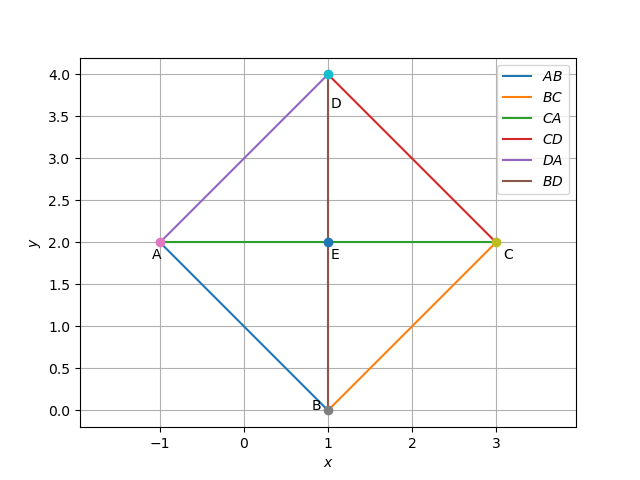
\includegraphics[width= \columnwidth]{solutions/1/4/quad.png}
\caption{Square ABCD}
\label{fig:2.2.7}
\end{figure}
See Fig. \ref{fig:2.2.7}.
The other two vertices can be obtained by using the following formula. 
\begin{align}
  \label{eq:square_points}
  \vec{B} = \frac{\norm{\vec{A}-\vec{C}}}{\sqrt{2}} \vec{P}\vec{e}_1+\vec{A}
  \\
  \vec{D} = \frac{\norm{\vec{A}-\vec{C}}}{\sqrt{2}} \vec{P}\vec{e}_2+\vec{A}
\end{align}
where 
\begin{align}
	\vec{P} = \myvec{\cos \brak{\theta-\frac{\pi}{4}} & \sin  \brak{\theta-\frac{\pi}{4}} \\ \sin \brak{\theta-\frac{\pi}{4}} & \cos \brak{\theta-\frac{\pi}{4}}}
\end{align}
and 



Let the given points be $\vec{A}, \vec{C}$.  The direction vector of the diagonal AC



\begin{enumerate}
\item From inspection we see that the opposite vertices forms a diagonal which is parallel to x-axis. Then the diagonal formed by other two vertices is parallel to y-axis(i.e. their x coordinates are equal). Let $\vec{A}= \myvec{-1\\2}$  and $\vec{C}=\myvec{3\\2}$. 

\item Diagonals bisect each other at 90\degree.
Let $\vec{B}$ and $\vec{D}$ be other two vertices. 
\item Using the property that diagonals bisect each other at 90\degree, we can obtain other vertices by rotating diagonal AC by 90\degree about $\vec{E}$ in clockwise or anticlockwise direction.

\item The rotation matrix for a rotation of angle 90\degree about origin in anticlockwise direction is given by
\begin{align}
\myvec{\cos90\degree&-\sin90\degree\\\sin90\degree&\cos90\degree}=\myvec{0&-1\\1&0}
\end{align}
The $\vec{E}$ is given by
\begin{align}
\vec{E}&= \frac{\vec{A}+\vec{C}}{2} \\
&= \myvec{1\\2}
\end{align}

\item To make the rotation we need to shift the $\vec{E}$ to origin. So the change in other vectors are
\begin{align}
\vec{A}-\vec{E}&=\myvec{-2\\0}\\
\vec{C}-\vec{E}&=\myvec{2\\0}
\end{align}

The required matrix now is $\myvec{-2&2\\0&0}$. Multiplying this with rotation matrix 
\begin{align}
&= \myvec{0&-1\\1&0}\myvec{-2&2\\0&0}\\
&=\myvec{0&0\\-2&2}
\end{align}
Now we obtained the coordinates as $\myvec{0\\-2}$ and $\myvec{0\\2}$.
To obtain the final coordinates we will add $\vec{E}$ to shift to the actual position.
\begin{align}
\vec{B}=\myvec{0\\-2}+\myvec{1\\2}\\
\vec{D}=\myvec{0\\2}+\myvec{1\\2}
\end{align}
Thus 
\begin{align}
\vec{B}&= \myvec{1\\0} \\
\vec{D}&= \myvec{1\\4}
\end{align} 
\item The python code for the figure can be downloaded from
\begin{lstlisting}
solutions/7/codes/quad/quad.py
\end{lstlisting}
\end{enumerate}  

%\end{enumerate}
%
\item  If 
$
\vec{a}=\myvec{1\\1\\1},
\vec{b}=\myvec{2\\-1\\3},
\vec{c}=\myvec{1\\-2\\1},
$
find a unit vector parallel to the vector $2\vec{a}-\vec{b}+3\vec{c}$.
\\
\solution 
\begin{figure}[!ht]
\centering
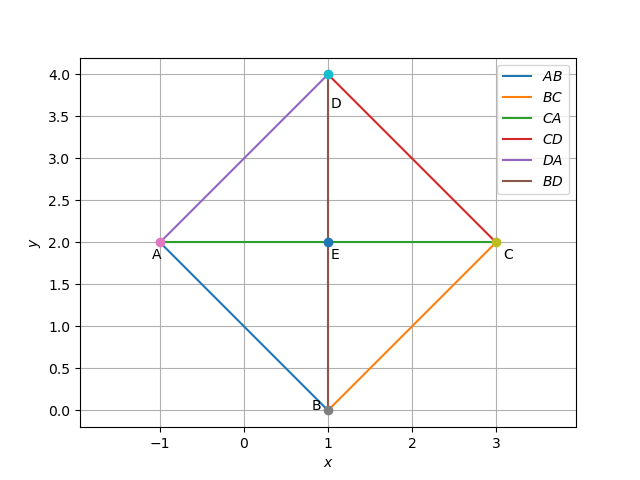
\includegraphics[width= \columnwidth]{solutions/1/4/quad.png}
\caption{Square ABCD}
\label{fig:2.2.7}
\end{figure}
See Fig. \ref{fig:2.2.7}.
The other two vertices can be obtained by using the following formula. 
\begin{align}
  \label{eq:square_points}
  \vec{B} = \frac{\norm{\vec{A}-\vec{C}}}{\sqrt{2}} \vec{P}\vec{e}_1+\vec{A}
  \\
  \vec{D} = \frac{\norm{\vec{A}-\vec{C}}}{\sqrt{2}} \vec{P}\vec{e}_2+\vec{A}
\end{align}
where 
\begin{align}
	\vec{P} = \myvec{\cos \brak{\theta-\frac{\pi}{4}} & \sin  \brak{\theta-\frac{\pi}{4}} \\ \sin \brak{\theta-\frac{\pi}{4}} & \cos \brak{\theta-\frac{\pi}{4}}}
\end{align}
and 



Let the given points be $\vec{A}, \vec{C}$.  The direction vector of the diagonal AC



\begin{enumerate}
\item From inspection we see that the opposite vertices forms a diagonal which is parallel to x-axis. Then the diagonal formed by other two vertices is parallel to y-axis(i.e. their x coordinates are equal). Let $\vec{A}= \myvec{-1\\2}$  and $\vec{C}=\myvec{3\\2}$. 

\item Diagonals bisect each other at 90\degree.
Let $\vec{B}$ and $\vec{D}$ be other two vertices. 
\item Using the property that diagonals bisect each other at 90\degree, we can obtain other vertices by rotating diagonal AC by 90\degree about $\vec{E}$ in clockwise or anticlockwise direction.

\item The rotation matrix for a rotation of angle 90\degree about origin in anticlockwise direction is given by
\begin{align}
\myvec{\cos90\degree&-\sin90\degree\\\sin90\degree&\cos90\degree}=\myvec{0&-1\\1&0}
\end{align}
The $\vec{E}$ is given by
\begin{align}
\vec{E}&= \frac{\vec{A}+\vec{C}}{2} \\
&= \myvec{1\\2}
\end{align}

\item To make the rotation we need to shift the $\vec{E}$ to origin. So the change in other vectors are
\begin{align}
\vec{A}-\vec{E}&=\myvec{-2\\0}\\
\vec{C}-\vec{E}&=\myvec{2\\0}
\end{align}

The required matrix now is $\myvec{-2&2\\0&0}$. Multiplying this with rotation matrix 
\begin{align}
&= \myvec{0&-1\\1&0}\myvec{-2&2\\0&0}\\
&=\myvec{0&0\\-2&2}
\end{align}
Now we obtained the coordinates as $\myvec{0\\-2}$ and $\myvec{0\\2}$.
To obtain the final coordinates we will add $\vec{E}$ to shift to the actual position.
\begin{align}
\vec{B}=\myvec{0\\-2}+\myvec{1\\2}\\
\vec{D}=\myvec{0\\2}+\myvec{1\\2}
\end{align}
Thus 
\begin{align}
\vec{B}&= \myvec{1\\0} \\
\vec{D}&= \myvec{1\\4}
\end{align} 
\item The python code for the figure can be downloaded from
\begin{lstlisting}
solutions/7/codes/quad/quad.py
\end{lstlisting}
\end{enumerate}  


\item Find a vector of magnitude 5 units, and parallel to the resultant of the vectors 
$
\vec{a}=\myvec{2\\3\\-1},
\vec{b}=\myvec{1\\-2\\1},
$
\\
\solution 
%\input./solutions/point_vector/13/solution.tex}
\item Show that the unit direction vector inclined equally to the coordinate axes is $\myvec{\frac{1}{\sqrt{3}}\\\frac{1}{\sqrt{3}}\\ \frac{1}{\sqrt{3}}}$.
\\
\solution 
%\input./solutions/point_vector/14/Latex/solution.tex}
\item Find a unit vector that makes an angle of $90\degree, 135\degree$ and $45\degree$ with the positive x, y and z axis respectively.
\solution 
%\input./solutions/point_vector/18/solution.tex}
\item Show that the line through the points \myvec{4\\7\\8}, \myvec{2\\3\\4} is parallel to the line through the points   \myvec{-1\\-2\\1}, \myvec{1\\2\\5}.
\\
\solution 
%\input./solutions/point_vector/21/solution.tex}
\item Find a vector $\vec{x}$ in the direction of \myvec{1\\-2} such that $\norm{\vec{x}} = 7$.
%
\solution Let $\vec{x} = k\myvec{1\\-2}$.  Then 
%
\begin{align}
\norm{\vec{x}} &= \abs{k}\norm{\myvec{1\\-2}}= 7
\\
\implies \abs{k} &= \frac{7}{\sqrt{5}}
\\
\text{or, } \vec{x} &= \frac{7}{\sqrt{5}}\myvec{1\\-2}
\end{align}
%
\item Find the direction vector of $PQ$, where 
\begin{align}
\vec{P} = \myvec{2\\3\\0},
\vec{Q} = \myvec{-1\\-2\\-4}
\end{align}
%
\solution The direction vector of $PQ$ is 
%
\begin{align}
\vec{P}-\vec{Q} = \myvec{3\\5\\4},
\end{align}
%
%\\
%\solution Choose $\vec{x} = \myvec{0\\y}$ and follow the approach in Problem \eqref{prob:line_perp_bisect}. Solve for $y$.

\item  Find the slope of a line, which passes through the origin, and the mid-point of the line segment joining the points $\vec{P} = \myvec{0\\ – 4}$ and $\vec{B} = \myvec{8\\ 0}$.
\solution 
%\input{./solutions/line_plane/24/solution.tex}
\item The slope of a line is double of the slope of another line. If the tangent of the angle
between them is $\frac{1}{3}$, find the slopes of the lines.
\solution 
%\input{./solutions/line_plane/25/solution.tex}
\item Find a unit vector that makes an angle of $90\degree, 60\degree$ and $30\degree$ with the positive x, y and z axis respectively.
%
\\
\solution
The direction vector is
%
\begin{align}
\label{eq:line_dir_cos}
\vec{x} &= \myvec{\cos 90\degree\\\cos 60\degree \\ \cos 30\degree} = \myvec{0 \\ \frac{1}{2}\\\frac{\sqrt{3}}{2}}
\end{align}
%
$\because \norm{\vec{x}}=1$, it is the desired unit vector.
\item Find the direction vectors and slopes of the lines passing through the points
%
\begin{enumerate}
\item \myvec{3\\-2} and \myvec{-1\\4}.
\item \myvec{3\\-2} and \myvec{7\\-2}.
\item \myvec{3\\-2} and \myvec{3\\4}.
\item Making an inclination of $60\degree$ with the positive direction of the x-axis.
\end{enumerate}
%
\solution
\begin{enumerate}
\item If the direction vector is 
\begin{align}
\myvec{1\\m}, 
\end{align}
%
the slope is $m$. Thus, the direction vector is
\begin{align}
\myvec{-1\\4} - \myvec{3\\-2} &= \myvec{-4\\6} = -\frac{1}{4} \myvec{-4\\6} 
\\
&=  \myvec{1\\-\frac{3}{2}} \implies m = -\frac{3}{2}
\end{align}
%
\item The direction vector is
\begin{align}
\myvec{7\\-2} - \myvec{3\\-2} &= \myvec{4\\0} 
\\
&=  \myvec{1\\0} \implies m = 0
\end{align}
%
\item The direction vector is
\begin{align}
\myvec{3\\4} - \myvec{3\\-2} &= \myvec{0\\6} 
\\
&=  \myvec{1\\ \infty} \implies m = \infty
\end{align}
%
\item The slope is $m = \tan 60 \degree = \sqrt{3}$ and the  direction vector is
\begin{align}
\myvec{1\\\sqrt{3}}
\end{align}
\end{enumerate}
\item If the angle between two lines is $\frac{\pi}{4}$ and the slope of one of the lines is $\frac{1}{4}$ find the slope of the other line.
\\
\solution The angle $\theta$ between two lines is given by 
%
\begin{align}
\tan \theta &= \frac{m_1-m_2}{1+m_1m_2}
\\
\implies 1 &= \frac{m_1-\frac{1}{4}}{1+\frac{m_1}{4}}
\\
\text{or } m_1 &= \frac{5}{3} 
\end{align}
%
%
%\\
%\solution 
%%Using \eqref{eq:tri_geo_ex_orth}
%\begin{align}
%\cbrak{\myvec{-2\\ 6}-\myvec{4\\8}}^T \cbrak{\myvec{8\\ 12}-\myvec{x\\24}}=  0 
%\end{align}
%%
%which can be used to obtain $x$.
\item If the points
$
\vec{A} = \myvec{6\\1}, 
\vec{B} = \myvec{8\\2}, 
\vec{C} = \myvec{9\\4}, 
\vec{D} = \myvec{p\\3}
$
are the vertices of a parallelogram, taken in order, find the value of $p$.
\\
\solution In the parallelogram $ABCD$, $AC$ and $BD$ bisect each other.  This can be used to find $p$.
\item Without using distance formula, show that points \myvec{– 2\\ – 1}, \myvec{4\\ 0}, \myvec{3\\ 3} and \myvec{–3\\ 2} are the vertices of a parallelogram.
\\
\solution
%\input{./solutions/5/chapters/quadrilateral/docq4.tex}

\item The two opposite vertices of a square are \myvec{-1\\2},  \myvec{3\\2}. Find the coordinates of the other two vertices.
\\
\solution
%\input{./solutions/7/chapters/quad/solution1.tex}

\item Find the direction vectors of the sides of a triangle with vertices
$
\vec{A} = \myvec{3\\5 \\-4},
\vec{B} = \myvec{-1\\1 \\2}, \text{ and }
\vec{C} = \myvec{-5\\ -5\\-2}
$
\\
\solution
%
%
\begin{align}
  \vec{A}-\vec{B} &= \myvec{0\\-1\\-2},
  \vec{A}-\vec{C} &= \myvec{-1\\-2\\0}
\end{align}
and 
\begin{align}
  \mydet{-1 & -2 \\-2 & 0} &= -4 \\
  \mydet{-2 & 0 \\0 & -1} &= 2 \\
  \mydet{0 & -1 \\-1 & -2} &= -1 \\
\end{align}
From   \eqref{eq:cross3d}, 
\begin{align}
  \frac{1}{2}\brak{\vec{A} - \vec{B}} \times \brak{\vec{A} - \vec{C}} = \frac{1}{2}\myvec{-4\\2\\-1}
\end{align}
and from \eqref{eq:cross3d}, the area of the triangle is
\begin{align}
  \frac{1}{2}\norm{\myvec{-4\\2\\-1}} = \frac{1}{2}\sqrt{4^2+2^2+1^2} = \frac{1}{2}\sqrt{21}
\end{align}

\item Find a unit vector in the direction of 
%
\begin{align}
\myvec{1\\1\\-2}.
\end{align}
%
\solution
%\input{solutions/aug/2/24.tex}

%
\item Find a unit vector in the direction of \myvec{2\\-1\\-2}.
\\
\solution
%\input{solutions/aug/2/21.tex}

%
%



\item Find a unit vector in the direction of the line passing through \myvec{-2\\4\\-5} and $\myvec{1\\2\\3}$.
%
\\
\solution
%\input{solutions/aug/2/22.tex}
\end{enumerate}
\section{Norm }
\renewcommand{\theequation}{\theenumi}
%\begin{enumerate}[label=\arabic*.,ref=\theenumi]
\begin{enumerate}[label=\thesection.\arabic*.,ref=\thesection.\theenumi]
\numberwithin{equation}{enumi}
\item Find a point on the x-axis, which is equidistant from the points \myvec{7\\ 6} and \myvec{3\\ 4}.
\\
\solution 
%\input./solutions/point_vector/22/solution.tex}
\item Write down a unit vector in the xy-plane, makeing an angle of $30\degree$ with the positive direction of the x-axis.
\\
\solution 
%\input./solutions/point_vector/25/solution.tex}

\item Find the value of $x$ for which $x\myvec{1\\1\\1}$ is a unit vector.
\\
\solution
%\input./solutions/point_vector/26/solution.tex}
\item If
\begin{align}
\vec{a} = \myvec{1\\2}, \vec{b} = \myvec{2\\1},
\end{align}
verify if  
\begin{enumerate}
\item $\norm{\vec{a}}=\norm{\vec{b}}$

\item $\vec{a}=\vec{b}$
\end{enumerate}
%
\solution
\begin{enumerate}
\item $\norm{\vec{a}}=\norm{\vec{b}},\vec{a}\ne\vec{b}$.
\end{enumerate}
\item Find a unit vector in the  direction of \myvec{2\\3\\1}.
%
\\
\solution The unit vector is given by 
\begin{align}
\frac{\myvec{2\\3\\1}}{\norm{\myvec{2\\3\\1}}} = \frac{1}{\sqrt{14}}\myvec{2\\3\\1}
\end{align}
\item Find the distance between the points
%
\begin{align}
\vec{P} = \myvec{1\\-3\\4},
\vec{Q} = \myvec{-4\\1\\2}
\end{align}
%
\solution 
\\
%%\input./solutions/line/geometry/examples/54/chapters/solution.tex}
%\input./solutions/point_vector/54/chapters/solution.tex}
The distance is given by $\norm{\vec{P}-\vec{Q}}$
\item Find $\norm{\vec{a}-\vec{b}}$, if 
\begin{align}
\norm{\vec{a}} = 2, 
\norm{\vec{b}} = 3,
\vec{a}^T\vec{b} = 4.
\end{align}
%
\solution 
%\input./solutions/point_vector/68/chapters/solution.tex}
%
%
%
\item If $\vec{a}$ is a unit vector and 
%
\begin{align}
\brak{\vec{x}-\vec{a}}\brak{\vec{x}+\vec{a}} = 8, 
\end{align}
%
then find $\vec{x}$.
%
\\
\solution 
%
\begin{align}
\brak{\vec{x}-\vec{a}}\brak{\vec{x}+\vec{a}} &= \norm{\vec{x}}^2-\norm{\vec{a}}^2
\\
\implies \norm{\vec{x}}^2 &= 9 \text{ or, } \norm{\vec{x}} = 3.
\end{align}
%
\item Find the point on the $x$-axis which is equidistant from 
\begin{align}
\myvec{2\\-5}, \myvec{-2\\9},
\end{align}
\solution
%\input./solutions/6/chapters/line/point_vector/solution.tex}
\item Find the values of $y$ for which the distance between the points 
\begin{align}
\vec{P} = \myvec{2\\-3}, \vec{Q} = \myvec{10\\y}
\end{align}
is 10 units.
\solution
%\input./solutions/7/chapters/line/point_vec/solution.tex}
\item A town B is located 36km east and 15 km north of the town A.  How would you find the distance from town A to town B without actually measuring it?
\\
\solution
%\input./solutions/3/chapters/line/towns/solution.tex}
\item Find the unit normal vector of the plane 
\begin{align}
\myvec{6 & -3 & -2}\vec{x}  = 1.
\end{align}
%
\solution The normal vector is 
%
\begin{align}
\vec{n} = \myvec{6 & -3 & -2}
\\
\because \norm{\vec{n}} = 7,
\end{align}
%
the unit normal vector is 
%
\begin{align}
\frac{\vec{n}}{\norm{\vec{n}}} = \frac{1}{7}\myvec{6 & -3 & -2}
\end{align}
%
%

\item Find the condition for $\vec{x} = \myvec{x_1\\x_2}$ to be equidistant from the points $\myvec{7\\1}, \myvec{3\\5}$.
\label{prob:line_perp_bisect}
%
\\
\solution From the given information,
%
\begin{align}
\norm{\vec{x}-\myvec{7\\1}}^2&=\norm{\vec{x}-\myvec{3\\5}}^2
\end{align}
\begin{multline}
\implies \norm{\vec{x}}^2 + \norm{\myvec{7\\1}}^2-2\myvec{7&1}\vec{x} 
\\= 
 \norm{\vec{x}}^2 + \norm{\myvec{3\\5}}^2-2\myvec{3&5}\vec{x} 
\end{multline}
%
which can be simplified to obtain
\begin{align}
\label{eq:line_p_bisect}
\myvec{1 & -1}\vec{x} = 2
\end{align}
%
which is the desired condition.  
The following code plots Fig. \ref{fig:line_perp_bisect}clearly showing that the above equation 
%\eqref{eq:line_p_bisect}
 is the perpendicular bisector of $AB$.

%
\begin{lstlisting}
codes/line/line_perp_bisect.py
\end{lstlisting}
%
%\begin{figure}[!ht]
%\includegraphics[width=\columnwidth]{./line/figs/line_perp_bisect.eps}
%\caption{}
%\label{fig:line_perp_bisect}
%\end{figure}
\item Find a point on the $y$-axis which is equidistant from the points $\vec{A} = \myvec{6\\5}, \vec{B} = \myvec{-4\\3}$.
\\
\solution
%\input{solutions/july/25/main1.tex}
\item Find the equation of set of points $\vec{P}$ such that
\begin{align}
PA^2+PB^2 =2k^2,
\end{align}
%
\begin{align}
\vec{A} = \myvec{3\\4 \\5},
\vec{B} = \myvec{-1\\3 \\-7},
\end{align}
%
respectively.
%
%
\solution
%\input{solutions/su2021/2/25.tex}   
\item Find the equation of the set of points $\vec{P}$ such that its distances from the points
$
\vec{A}=\myvec{3\\4\\-5}, 
\vec{B}=\myvec{-2\\1\\4}
$
are equal. 
\\
\solution
%\input{solutions/su2021/2/29/main.tex}
\end{enumerate}
\section{Section}
\renewcommand{\theequation}{\theenumi}
%\begin{enumerate}[label=\arabic*.,ref=\theenumi]
\begin{enumerate}[label=\thesection.\arabic*.,ref=\thesection.\theenumi]
\numberwithin{equation}{enumi}


\item Find $\vec{R}$ which divides the line joining the points 
\begin{align}
\vec{P} = 2\vec{a}+\vec{b}
\\
\vec{Q} = \vec{a}-\vec{b}
\end{align}
externally in the ratio $1:2$.
\item If 
\begin{align}
\vec{P} = 3\vec{a}-2\vec{b}
\\
\vec{Q} = \vec{a}+\vec{b}
\end{align}
%
find $\vec{R}$, which divides $PQ$ in the ratio $2:1$
\begin{enumerate}
\item internally,
\item externally.
\end{enumerate}
%
\solution
%\input{solutions/sep/20.tex}
\item Draw a line segement of length 7.6 cm and divide it in the ratio $5:8$.
\\
\solution Let the end points of the line be 
\begin{align}
\vec{A} = \myvec{0\\0}, \vec{B} = \myvec{7.6\\0}
\end{align}
Using section formula, 
%From \eqref{eq:tri_geo_ex_caorth_section},
the point $\vec{C}$
\begin{align}
\label{eq:line_section_form}
\vec{C} = \frac{k \vec{B} + \vec{A}}{k+1}
\end{align}
If $\vec{C}$ divides $AB$ in the ratio 
\begin{align}
 m = \frac{5}{8},
\end{align}
then,
\begin{align}
\label{eq:line_section_form_m}
\frac{\norm{\vec{C}-\vec{A}}^2}{\norm{\vec{B}-\vec{C}}^2} &= m^2
\\
\implies \frac{\frac{k^2\norm{\vec{B}-\vec{A}}^2}{\brak{k+1}^2}}{\frac{\norm{\vec{B}-\vec{A}}^2}{\brak{k+1}^2}} &=m^2
\\
\implies k = m &
\end{align}
upon substituting from \eqref{eq:line_section_form_m} and simplifying. \eqref{eq:line_section_form} is known as the section formula.
%
The following code plots Fig. \ref{fig:section}
\begin{lstlisting}
codes/line/draw_section.py
\end{lstlisting}
		%\begin{figure}[!ht]
		%\includegraphics[width=\columnwidth]{./line/figs/section.eps}
		%\caption{}
		%\label{fig:section}
		%\end{figure}
\item Find the coordinates of the point which divides the line segment joining the points \myvec{4\\-3} and \myvec{8\\5} in the ratio $3:1$ internally.
\\
\solution Using \eqref{eq:line_section_form},
the desired point is 
\begin{align}
\vec{P} = \frac{3 \myvec{4\\-3} + \myvec{8\\5}}{4}
\end{align}
\item In what ratio does the point \myvec{-4\\6} divide the line segment joining the points 
%
\begin{align}
\vec{A} = \myvec{-6\\10},
\vec{B} = \myvec{3\\-8}
\end{align}
%
\\
\solution Use \eqref{eq:line_section_form}.
\item Find the coordinates of the points of trisection of the line segement joining the points
%
\begin{align}
\vec{A} = \myvec{2\\-2},
\vec{B} = \myvec{-7\\4}
\end{align}
%
\\
\solution Using \eqref{eq:line_section_form}, the coordinates are
%
\begin{align}
\label{eq:line_section_form_tri}
\vec{P} &= \frac{2 \vec{A} + \vec{B}}{3}
\\
\vec{Q} &= \frac{ \vec{A} + 2\vec{B}}{3}
\end{align}
%
\item Find the ratio in which the y-axis divides the line segment joining the points \myvec{5\\-6} and \myvec{-1\\-4}.
\\
\solution Let the corresponding point on the $y$-axis be$\myvec{0\\y}$. If the ratio be $k:1$,
using \eqref{eq:line_section_form}, the coordinates are
%
\begin{align}
\myvec{0\\y} &= k\myvec{5\\-6}+ \myvec{-1\\-4}
\\
\implies 0 &= 5k-1 \implies k = \frac{1}{5}
\end{align}
%
\item Find the coordinates of the point which divides the join of 
\begin{align}
\myvec{-1\\7},  \myvec{4\\-3}
%\vec{P} = \myvec{2\\-3}, \vec{Q} = \myvec{10\\y}
\end{align}
%
in the ratio $2:3$.
\\
\solution
%\input{./solutions/1/chapters/line/point_line/solution.tex}

\item Find the coordinates of the points of trisection of the line segment joining \myvec{4\\-1} and \myvec{-2\\-3}.
\\
\solution
%\input{./solutions/2/chapters/line_ex/pts_on_a_line/solution.tex}
\item Find the ratio in which the line segment joining the points \myvec{-3\\10} and \myvec{6\\-8} is divided by \myvec{-1\\6}.
\\
\solution
%\input{./solutions/3/chapters/line/section/solution.tex}
\item Find the ratio in whcih the line segment joining $\vec{A}=\myvec{1\\-5}, \vec{B}=\myvec{-4\\5}$ is divided by the $x$-axis.  Also find the coordinates of the point of division.
\\
\solution
%\input{./solutions/4/chapters/line/point_on_line/solution.tex}
\item If \myvec{1\\2}, \myvec{4\\y}, \myvec{x\\6} and \myvec{3\\5} are the vertices of a parallelogram taken in order, find $x$ and $y$.
\\
\solution
%\input{./solutions/5/chapters/lines/docq10.tex}
\item If $\vec{A}=\myvec{-2\\-2}, \vec{B}=\myvec{2\\-4}$ respectively, find the coordinates of $\vec{P}$ such that $AP = \frac{3}{7}AB$ and $\vec{P}$ lies on the line segment $AB$.
\\
\solution
%\input{./solutions/6/chapters/line/point_line/solution.tex}
\item Find the coordinates of the points which divide the line segment joining $\vec{A}=\myvec{-2\\2}, \vec{B}=\myvec{2\\8}$ into four equal parts.
\\
\solution
%\input{./solutions/7/chapters/line/point_line/solution.tex}
\end{enumerate}
\section{Projection}
\renewcommand{\theequation}{\theenumi}
%\begin{enumerate}[label=\arabic*.,ref=\theenumi]
\begin{enumerate}[label=\thesection.\arabic*.,ref=\thesection.\theenumi]
\numberwithin{equation}{enumi}
\item Find the projection of the vector 
\begin{align}
\myvec{1\\3\\7}
\end{align}
on the vector
\begin{align}
\myvec{7\\-1\\8}
\end{align}
\\
\solution 
%\input./solutions/point_vector/24/solution.tex}
\item Find the projection of the vector 
\begin{align}
\vec{a} = \myvec{2\\3\\2}
\end{align}
on the vector
\begin{align}
\vec{b}=\myvec{1\\2\\1}.
\end{align}
%
\solution The projection of $\vec{a}$ on $\vec{b}$ is shown in Fig. \ref{fig:line_proj}. It has magnitude $\norm{\vec{a}}\cos \theta$ and is in the direction of $\vec{b}$.
%
%
%\begin{figure}
%\centering
%\includegraphics[width=\columnwidth]{./line/figs/line_proj.eps}
%\caption{}
%\label{fig:line_proj}
%\end{figure}
%
Thus, the projection is defined as 
\begin{align}
\brak{\norm{\vec{a}}\cos\theta} \frac{\vec{b}}{\norm{\vec{b}}}
=  \frac{\brak{\vec{a}^T\vec{b}}\norm{\vec{a}}}{\norm{\vec{b}}}\vec{b}
\end{align}
\end{enumerate}
\section{Applications}
\renewcommand{\theequation}{\theenumi}
%\begin{enumerate}[label=\arabic*.,ref=\theenumi]
\begin{enumerate}[label=\thesection.\arabic*.,ref=\thesection.\theenumi]
\numberwithin{equation}{enumi}
\item Find the perpendicular distances of the following lines from the origin and angle between the perpendicular and the positive x-axis.
\begin{enumerate}
\item $\myvec{1 & -\sqrt{3}}\vec{x} = -8$.
\item $\myvec{0 & 1}\vec{x} = 2$.
\item $\myvec{1 & -1}\vec{x} = 4$.
\end{enumerate}

\item Find $\norm{\vec{a}}$ and $\norm{\vec{b}}$ if 
\begin{align}
\brak{\vec{a}+\vec{b}}^T\brak{\vec{a}-\vec{b}} &= 8
\\
\norm{\vec{a}}&=8\norm{\vec{b}}
\end{align}
\item Evaluate the product 
\begin{align}
\brak{3\vec{a}-5\vec{b}}^T\brak{2\vec{a}+7\vec{b}} 
\end{align}
\item Find $\norm{\vec{a}}$ and $\norm{\vec{b}}$, if
\begin{align}
\norm{\vec{a}} &= \norm{\vec{b}},
\\
\vec{a}^T\vec{b} = \frac{1}{2} 
\end{align}
and the angle between $\vec{a}$ and $\vec{b}$ is $60\degree$.
\item Show that 
\begin{align}
\brak{\norm{\vec{a}}\vec{b}+\norm{\vec{b}}\vec{a}}\perp \brak{\norm{\vec{a}}\vec{b}-\norm{\vec{b}}\vec{a}}\\
\end{align}
\item If $\vec{a}^T\vec{a}=0$ and  $\vec{a}\vec{b}=0$, what can be concluded about the vector $\vec{b}$?
\item If $\vec{a},\vec{b},\vec{c}$ are unit vectors such that 
\begin{align}
\vec{a}+\vec{b}+\vec{c} = 0,
\end{align}
find the value of 
\begin{align}
\vec{a}^T\vec{b}+\vec{b}^T\vec{c}+\vec{c}^T\vec{a}.
\end{align}
\item If $\vec{a} \ne \vec{0}, \lambda \ne 0$, then $\norm{\lambda \vec{a}} = 1$ if
\begin{enumerate}
\item $\lambda =1$
\item $\lambda = -1$
\item $\norm{\vec{a}}=\abs{\lambda}$
\item $\norm{\vec{a}}=\frac{1}{\abs{\lambda}}$
\end{enumerate}
\item If a unit vector $\vec{a}$ makes angles $\frac{\pi}{3}$ with the x-axis and $\frac{\pi}{4}$ with the y-axis and an acute angle $\theta$ with the z-axis, find $\theta$ and $\vec{a}$.
\item Show that 
\begin{align}
\brak{\vec{a}-\vec{b}}\times \brak{\vec{a}+\vec{b}} = 2\brak{\vec{a}\times\vec{b}}
\end{align}
\item If $\vec{a}^T\vec{b} = 0$ and $\vec{a}\times \vec{b}$ = 0, what can you conclude about $\vec{a}$ and $\vec{b}$?
\item Find $\vec{x}$ if  $\vec{a}$ is a unit vector such that
\begin{align}
\brak{\vec{x}-\vec{a}}^T\brak{\vec{x}+\vec{a}} = 12.
\end{align}
\item If $\norm{\vec{a}} = 3, \norm{\vec{b}} =\frac{\sqrt{2}}{3}$, then $\vec{a}\times \vec{b}$ is a unit vector if the angle between $\vec{a}$ and $\vec{b}$ is 
\begin{enumerate}[itemsep = 2pt]
\begin{multicols}{2}
\item $\frac{\pi}{6}$
\item $\frac{\pi}{4}$
\item $\frac{\pi}{3}$
\item $\frac{\pi}{2}$
\end{multicols}
\end{enumerate}
\item Prove that 
\begin{align}
\brak{\vec{a}+\vec{b}}^T\brak{\vec{a}+\vec{b}} &= \norm{\vec{a}}^2+\norm{\vec{b}}^2
\\
\iff \vec{a}&\perp\vec{b}.
\end{align}
\item If $\theta$ is the angle between two vectors $\vec{a}$ and $\vec{b}$, then $\vec{a}^T\vec{b} \ge $ only when 
\begin{enumerate}[itemsep = 2pt]
\begin{multicols}{2}
\item $0 < \theta < \frac{\pi}{2}$
\item $0 \le \theta \le \frac{\pi}{2}$
\item $0 < \theta < {\pi}$
\item $0 \le \theta \le {\pi}$
\end{multicols}
\end{enumerate}
\item Let $\vec{a}$ and $\vec{b}$ be two unit vectors and $\theta$ be the angle between them.  Then $\vec{a}+\vec{b}$ is a unit vector if 
\begin{enumerate}[itemsep = 2pt]
\begin{multicols}{2}
\item $\theta = \frac{\pi}{4}$
\item $\theta = \frac{\pi}{3}$
\item $\theta = \frac{\pi}{2}$
\item $\theta = \frac{2\pi}{3}$
\end{multicols}
\end{enumerate}
\item If $\theta$ is the angle between any two vectors $\vec{a}$ and $\vec{b}$, then 
$\norm{\vec{a}^T\vec{b}} = \norm{\vec{a} \times \vec{b}}$ when $\theta$ is equal to 
\begin{enumerate}[itemsep = 2pt]
\begin{multicols}{2}
\item 0
\item $\frac{\pi}{4}$
\item $\frac{\pi}{2}$
\item $\pi$.
\end{multicols}
\end{enumerate}
\item A bullet fired at an angle of 30$\degree$ with the horizontal hits the ground 3.0 km away. By adjusting its angle of projection, can one hope to hit a target 5.0 km away ? Assume the muzzle speed to be fixed, and neglect air resistance.
\item  A fighter plane flying horizontally at an altitude of 1.5 km with speed 720 km/h passes directly overhead an anti-aircraft gun. At what angle from the vertical should the gun be fired for the shell with muzzle speed 600 $m s^{-1}$ to hit the plane ? 
At what minimum  altitude should the pilot fly the plane to avoid being hit ? (Take g = 10$ m s^{-2}$
).
\item Consider the collision depicted in Fig. \ref{fig:6.10} to be between two billiard balls with equal masses $m_1= m_2$.  The first ball is called the cue while the second ball is called the target. The billiard player wants to 'sink' the target ball in a corner pocket, which is at an angle $\theta_2=37\degree$.  Assume that the collosion
is elastic and that friction and rotational motion are not important. Obtain $\theta_1$.
%\begin{figure}[!ht]
%\centering
%\includegraphics[width=\columnwidth]{./line/figs/11-1/6/6.10.eps}
%\caption{}
%\label{fig:6.10}
%\end{figure}
\item Rain is falling vertically with a speed of 35 $m s^{-1}$
. Winds starts blowing after sometime with a speed of 12 $m s^{-1}$ in
east to west direction. In which direction should a boy waiting at a bus stop hold his umbrella ?
%
\\
\solution 
%\input{./solutions/1/chapters/line/Motion_plane/solution.tex}

\item A motorboat is racing towards north at 25 km/h and the water current in that region is 10 km/h in the direction of 60$\degree$ east of south. Find the resultant velocity of the boat.
\\
\solution 
%\input{./solutions/2/chapters/line_ex/motion_in_a_plane/solution.tex}
\item Rain is falling vertically with a speed of 35 $m s^{-1}$
. A woman rides a bicycle with a speed of 12 $ms^{-1}$ in east to west
direction. What is the direction in which she should hold her umbrella ?
\\
\solution 
%\input{./solutions/3/chapters/line/rain/solution.tex}
\item  A hiker stands on the edge of a cliff 490 m above the ground and throws a stone horizontally with an initial speed of 15 $m s^{-1}$
. Neglecting air resistance,
find the time taken by the stone to reach the ground, and the speed with which it hits the ground. (Take g = 9.8 $m s^{-2}$
).
\\
\solution 
%\input{./solutions/4/chapters/line/motion/solution.tex}
\item Rain is falling vertically with a speed of 30 $m s^{-1}$. A woman rides a bicycle with a speed  of 10 $m s^{-1}$ in the north to south direction. What is the direction in which she should
hold her umbrella?
\\
\solution 
%\input{./solutions/5/chapters/lines/docq12.tex}
\item A man can swim with a speed of 4.0 km/h in still water. How long does he take to cross a river 1.0 km wide if the river flows steadily at 3.0 km/h and he makes his strokes normal to the river current? How far down the river does he go when he reaches the other bank ?
\\
\solution 
%\input{./solutions/6/chapters/line/motion_plane/solution.tex}
\item In a harbour, wind is blowing at the speed of 72 km/h and the flag on the mast of a boat anchored in the harbour flutters along the N-E direction. If the boat starts moving at a speed of 51 km/h to the north, what is the direction of the flag on the mast of the boat ?
\\
\solution 
%\input{./solutions/7/chapters/line/motion/solution.tex}

\item Find the intercepts cut off by the plane 
$
\myvec{2 & 1 & 1}\vec{x}=5.
$
\end{enumerate}
\section{Locus}
\renewcommand{\theequation}{\theenumi}
%\begin{enumerate}[label=\arabic*.,ref=\theenumi]
\begin{enumerate}[label=\thesection.\arabic*.,ref=\thesection.\theenumi]
\numberwithin{equation}{enumi}
\item The sum of the perpendicular distances of a variable point $\vec{P}$ from the lines
%
\begin{align}
\myvec{1 & 1}\vec{x} &= 0
\\
\myvec{3 & -2}\vec{x} &= -7
\end{align}
%
is always 10.  Show that $\vec{P}$ must move on a line.
\end{enumerate}
\end{document}


